\documentclass{beamer}

\mode<presentation> {

% The Beamer class comes with a number of default slide themes
% which change the colors and layouts of slides.
\usetheme{Montpellier}

% As well as themes, the Beamer class has a number of color themes
% for any slide theme.
\usecolortheme{dove}

%\setbeamertemplate{footline} % To remove the footer line in all slides uncomment this line
%\setbeamertemplate{footline}[page number] % To replace the footer line in all slides with a simple slide count uncomment this line

\setbeamertemplate{navigation symbols}{} % To remove the navigation symbols from the bottom of all slides uncomment this line
}

\usepackage{graphicx} % Required for displaying images
\graphicspath{{./images/}} % Directory for finding images
\DeclareGraphicsExtensions{.png,.pdf} % Try .png before trying .pdf
\usepackage{caption}
\captionsetup[figure]{labelformat=empty}% redefines the caption setup of the figures environment in the beamer class.
\usepackage{subcaption}

%----------------------------------------------------------------------------------------
%	TITLE PAGE
%----------------------------------------------------------------------------------------

\title[Java Stratopolis]{A Java Implementation of Stratopolis} % The short title appears at the bottom of every slide, the full title is only on the title page
\author{Yuxi Liu}
\date{19 October, 2016}

\begin{document}

\begin{frame}
\titlepage % Print the title page as the first slide
\end{frame}

%----------------------------------------------------------------------------------------
%	PRESENTATION SLIDES
%----------------------------------------------------------------------------------------

\begin{frame}
\frametitle{UML (1 minute)}
\begin{figure}
\includegraphics[width=0.6\linewidth]{uml}
\end{figure}
\end{frame}

\begin{frame}
\frametitle{UML (1 minute)}
\begin{figure}
\includegraphics[width=1.1\linewidth]{uml_simple}
\end{figure}
\end{frame}

\begin{frame}
\frametitle{GameField class (2 minute)}
The GameField class represents the game board. It can decide whether a piece can be played on the board, and it can score the board.

A Gamefield has three matrices, representing color, height, and index.
\tiny\[
  \begin{bmatrix}
    B & B & B & B & B & B \\ 
    B & B & R & B & B & B \\ 
    B & B & G & B & B & B \\ 
    B & B & B & B & B & B
  \end{bmatrix}
  \begin{bmatrix}
    0 & 0 & 0 & 0 & 0 & 0 \\ 
    0 & 0 & 1 & 0 & 0 & 0 \\ 
    0 & 0 & 1 & 0 & 0 & 0 \\ 
    0 & 0 & 0 & 0 & 0 & 0
  \end{bmatrix}
  \begin{bmatrix}
    -1 & -1 & -1 & -1 & -1 & -1 \\ 
    -1 & -1 &  0 & -1 & -1 & -1 \\ 
    -1 & -1 &  0 & -1 & -1 & -1 \\ 
    -1 & -1 & -1 & -1 & -1 & -1
  \end{bmatrix}
\]
\begin{figure}
\includegraphics[width=0.4\linewidth]{0}
\end{figure}
\end{frame}

\begin{frame}
\frametitle{GameField class (2 minute)}
The GameField class represents the game board. It can decide whether a piece can be played on the board, and it can score the board.

A Gamefield has three matrices, representing color, height, and index.
\tiny\[
  \begin{bmatrix}
    B & B & G & B & B & B \\ 
    B & B & R & G & B & B \\ 
    B & B & G & B & B & B \\ 
    B & B & B & B & B & B
  \end{bmatrix}
  \begin{bmatrix}
    0 & 0 & 1 & 1 & 0 & 0 \\ 
    0 & 0 & 1 & 1 & 0 & 0 \\ 
    0 & 0 & 1 & 0 & 0 & 0 \\ 
    0 & 0 & 0 & 0 & 0 & 0
  \end{bmatrix}
  \begin{bmatrix}
    -1 & -1 &  1 &  1 & -1 & -1 \\ 
    -1 & -1 &  0 &  1 & -1 & -1 \\ 
    -1 & -1 &  0 & -1 & -1 & -1 \\ 
    -1 & -1 & -1 & -1 & -1 & -1
  \end{bmatrix}
\]
\begin{figure}
\includegraphics[width=0.4\linewidth]{1}
\end{figure}
\end{frame}

\begin{frame}
\frametitle{GameField class (2 minute)}
The GameField class represents the game board. It can decide whether a piece can be played on the board, and it can score the board.

A Gamefield has three matrices, representing color, height, and index.
\tiny\[
  \begin{bmatrix}
    B & B & G & B & B & B \\ 
    B & R & R & G & B & B \\ 
    B & B & G & B & B & B \\ 
    B & B & B & B & B & B
  \end{bmatrix}
  \begin{bmatrix}
    0 & 0 & 1 & 1 & 0 & 0 \\ 
    0 & 1 & 1 & 1 & 0 & 0 \\ 
    1 & 1 & 1 & 0 & 0 & 0 \\ 
    0 & 0 & 0 & 0 & 0 & 0
  \end{bmatrix}
  \begin{bmatrix}
    -1 & -1 &  1 &  1 & -1 & -1 \\ 
    -1 &  2 &  0 &  1 & -1 & -1 \\ 
     2 &  2 &  0 & -1 & -1 & -1 \\ 
    -1 & -1 & -1 & -1 & -1 & -1
  \end{bmatrix}
\]
\begin{figure}
\includegraphics[width=0.4\linewidth]{2}
\end{figure}
\end{frame}

\begin{frame}
\frametitle{GameField class (2 minute)}
The GameField class represents the game board. It can decide whether a piece can be played on the board, and it can score the board.

A Gamefield has three matrices, representing color, height, and index.
\tiny\[
  \begin{bmatrix}
    B & B & G & B & B & B \\ 
    B & R & R & G & R & B \\ 
    B & B & G & G & G & B \\ 
    B & B & B & B & B & B
  \end{bmatrix}
  \begin{bmatrix}
    0 & 0 & 1 & 1 & 0 & 0 \\ 
    0 & 1 & 1 & 1 & 1 & 0 \\ 
    1 & 1 & 1 & 1 & 1 & 0 \\ 
    0 & 0 & 0 & 0 & 0 & 0
  \end{bmatrix}
  \begin{bmatrix}
    -1 & -1 &  1 &  1 & -1 & -1 \\ 
    -1 &  2 &  0 &  1 &  3 & -1 \\ 
     2 &  2 &  0 &  3 &  3 & -1 \\ 
    -1 & -1 & -1 & -1 & -1 & -1
  \end{bmatrix}
\]
\begin{figure}
\includegraphics[width=0.4\linewidth]{3}
\end{figure}
\end{frame}

\begin{frame}
\frametitle{GameField class (2 minute)}
The GameField class represents the game board. It can decide whether a piece can be played on the board, and it can score the board.

A Gamefield has three matrices, representing color, height, and index.
\tiny\[
  \begin{bmatrix}
    R & B & G & B & B & B \\ 
    R & R & R & G & R & B \\ 
    B & B & G & G & G & B \\ 
    B & B & B & B & B & B
  \end{bmatrix}
  \begin{bmatrix}
    1 & 1 & 1 & 1 & 0 & 0 \\ 
    1 & 1 & 1 & 1 & 1 & 0 \\ 
    1 & 1 & 1 & 1 & 1 & 0 \\ 
    0 & 0 & 0 & 0 & 0 & 0
  \end{bmatrix}
  \begin{bmatrix}
     4 &  4 &  1 &  1 & -1 & -1 \\ 
     4 &  2 &  0 &  1 &  3 & -1 \\ 
     2 &  2 &  0 &  3 &  3 & -1 \\ 
    -1 & -1 & -1 & -1 & -1 & -1
  \end{bmatrix}
\]
\begin{figure}
\includegraphics[width=0.4\linewidth]{4}
\end{figure}
\end{frame}

\begin{frame}
\frametitle{GameField class (2 minute)}
The GameField class represents the game board. It can decide whether a piece can be played on the board, and it can score the board.

A Gamefield has three matrices, representing color, height, and index.
\tiny\[
  \begin{bmatrix}
    R & B & G & B & B & B \\ 
    R & R & R & G & R & B \\ 
    B & B & G & G & G & G \\ 
    B & B & B & B & G & G
  \end{bmatrix}
  \begin{bmatrix}
    1 & 1 & 1 & 1 & 0 & 0 \\ 
    1 & 1 & 1 & 1 & 1 & 0 \\ 
    1 & 1 & 1 & 1 & 1 & 1 \\ 
    0 & 0 & 0 & 0 & 1 & 1
  \end{bmatrix}
  \begin{bmatrix}
     4 &  4 &  1 &  1 & -1 & -1 \\ 
     4 &  2 &  0 &  1 &  3 & -1 \\ 
     2 &  2 &  0 &  3 &  3 &  5 \\ 
    -1 & -1 & -1 & -1 &  5 &  5
  \end{bmatrix}
\]
\begin{figure}
\includegraphics[width=0.4\linewidth]{5}
\end{figure}
\end{frame}

\begin{frame}
\frametitle{GameField class (2 minute)}
The GameField class represents the game board. It can decide whether a piece can be played on the board, and it can score the board.

A Gamefield has three matrices, representing color, height, and index.
\tiny\[
  \begin{bmatrix}
    R & R & B & B & B & B \\ 
    R & R & R & G & R & B \\ 
    B & B & G & G & G & G \\ 
    B & B & B & B & G & G
  \end{bmatrix}
  \begin{bmatrix}
    1 & 2 & 2 & 1 & 0 & 0 \\ 
    1 & 1 & 2 & 1 & 1 & 0 \\ 
    1 & 1 & 1 & 1 & 1 & 1 \\ 
    0 & 0 & 0 & 0 & 1 & 1
  \end{bmatrix}
  \begin{bmatrix}
     4 &  6 &  6 &  1 & -1 & -1 \\ 
     4 &  2 &  6 &  1 &  3 & -1 \\ 
     2 &  2 &  0 &  3 &  3 &  5 \\ 
    -1 & -1 & -1 & -1 &  5 &  5
  \end{bmatrix}
\]
\begin{figure}
\includegraphics[width=0.4\linewidth]{6}
\end{figure}
\end{frame}

\begin{frame}
\frametitle{GameField class (2 minute)}
The GameField class represents the game board. It can decide whether a piece can be played on the board, and it can score the board.

A Gamefield has three matrices, representing color, height, and index.
\tiny\[
  \begin{bmatrix}
    R & R & B & B & B & B \\ 
    R & R & R & G & R & G \\ 
    B & B & G & G & G & G \\ 
    B & B & B & B & G & G
  \end{bmatrix}
  \begin{bmatrix}
    1 & 2 & 2 & 1 & 1 & 1 \\ 
    1 & 1 & 2 & 1 & 1 & 1 \\ 
    1 & 1 & 1 & 1 & 1 & 1 \\ 
    0 & 0 & 0 & 0 & 1 & 1
  \end{bmatrix}
  \begin{bmatrix}
     4 &  6 &  6 &  1 &  7 &  7 \\ 
     4 &  2 &  6 &  1 &  3 &  7 \\ 
     2 &  2 &  0 &  3 &  3 &  5 \\ 
    -1 & -1 & -1 & -1 &  5 &  5
  \end{bmatrix}
\]
\begin{figure}
\includegraphics[width=0.4\linewidth]{7}
\end{figure}
\end{frame}

\begin{frame}
\frametitle{GameField class (2 minute)}
The GameField class represents the game board. It can decide whether a piece can be played on the board, and it can score the board.

A Gamefield has three matrices, representing color, height, and index.
\tiny\[
  \begin{bmatrix}
    R & R & B & B & B & B \\ 
    R & R & R & G & R & G \\ 
    R & R & G & G & G & G \\ 
    B & B & B & B & G & G
  \end{bmatrix}
  \begin{bmatrix}
    1 & 2 & 2 & 1 & 1 & 1 \\ 
    2 & 1 & 2 & 1 & 1 & 1 \\ 
    2 & 2 & 1 & 1 & 1 & 1 \\ 
    0 & 0 & 0 & 0 & 1 & 1
  \end{bmatrix}
  \begin{bmatrix}
     4 &  6 &  6 &  1 &  7 &  7 \\ 
     8 &  2 &  6 &  1 &  3 &  7 \\ 
     8 &  8 &  0 &  3 &  3 &  5 \\ 
    -1 & -1 & -1 & -1 &  5 &  5
  \end{bmatrix}
\]
\begin{figure}
\includegraphics[width=0.4\linewidth]{8}
\end{figure}
\end{frame}

\begin{frame}
\frametitle{GUI screenshot (10 seconds)}
\begin{figure}
\includegraphics[width=0.7\linewidth]{gui_screenshot}
\end{figure}
\end{frame}

\begin{frame}
\frametitle{Connected Component Labelling (1 minutes)}
To score the board, we must solve the algorithmically interesting problem: how to find out the connected color regions of a board?

\begin{figure}[h!]
\centering
\begin{subfigure}[t]{.5\textwidth}
  \centering
  \includegraphics[width=.7\linewidth]{before_ccl}
  \caption{Input: the color matrix}
\end{subfigure}%
\begin{subfigure}[t]{.5\textwidth}
  \centering
  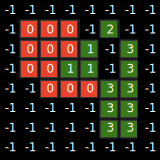
\includegraphics[width=.7\linewidth]{after_ccl}
  \caption{Output: the component label matrix.}
\end{subfigure}
\caption{Connected Component Labelling. The background gets label -1.}
\end{figure}

\end{frame}

\begin{frame}
\frametitle{2 Pass Union-find CCL Algorithm (20 seconds)}
We used a two pass algorithm that uses an implementation of the set ADT, called ``union-find''. 

Solves the problem in linear space and nearly in linear time. 
\begin{figure}
\includegraphics[width=0.9\linewidth]{ccl_algo}
\caption{{\tiny{}Pictures copied from http://aishack.in/tutorials/labelling-connected-components-example/}}
\end{figure}

Search ``union find connected components labelling'' for details.
\end{frame}

\begin{frame}
\frametitle{Base64 encoding (20 seconds)}
We implemented game saving and loading by converting the game state into a single savestring, which can later be loaded to recreate the game state. 
\begin{figure}
\includegraphics[width=\linewidth]{base64_conversion}
\end{figure}
The savestring is encoded in Base64 to discourage cheating.
\end{frame}

\begin{frame}
\frametitle{Demonstration (4 minutes)}
Green is human, red is OneLookaheadPlayer.

Demonstrate error warning, move highlighting, forward and backward stepping, savestring, help screen, and credit screen.
\end{frame}

\begin{frame}
\frametitle{Q\&{}A (1 minute)}
Any questions?
\end{frame}

%----------------------------------------------------------------------------------------

\end{document} 
